\documentclass[../main.tex]{subfiles}


\begin{document}
%\begin{center}
%\begin{tabularx}{\textwidth}{|1|X|}
\begin{longtable}{| p{.20\textwidth} | p{.80\textwidth} |} 
\hline
    Kratak opis &  Klijent dolazi na zakazan trening u teretanu. Predaje svoju člansku kartu recepcionaru i odlazi na trening. Recepcionar unosi dolazak i sistem se ažurira.\\ 
\hline    
    Učesnici & \begin{enumerate}
        \item Klijent – Želi da brzo uđe na trening, bez čekanja.
        \item Recepcionar – Želi da brzo i efikasno zabeleži sve klijente koji su došli, kao i da u sistemu uvek bude ispravan broj dolazaka.   
     \end{enumerate}\\
\hline
   Preduslovi & \begin{enumerate}
       \item Sistem je u funkciji.
       \item Klijent ima uplaćenu odgovarajuću članarinu.
       \item Klijent ima zakazan trening.
   \end{enumerate}\\
\hline  
    Postuslovi & \begin{enumerate}
        \item Ažurirani su podaci o dolascima korisnika na njegovom profilu.
        \item Ažurirana je posećenost odgovarajućeg treninga.
    \end{enumerate}\\
\hline
    Osnovni tok & \begin{enumerate}
        \item Klijent dolazi na recepciju i predaje svoju člansku kartu.
        \item Recepcionar unosi broj članske karte u deo sistema za evidenciju dolazaka.
        \item Sistem izlistava zakazane i uplaćene treninge klijenta.
        \item Recepcionar obeležava trening na koji je klijent došao. Pritiska dugme „Potvrdi dolazak“.
        \item Sistem čuva izmenu. Obaveštava da je sačuvana izmena.
        \item Recepcionar obaveštava klijenta da je evidentiran dolazak.
        \item Klijent odlazi na trening.
    \end{enumerate}\\
\hline
    Alternativni tokovi & \begin{itemize}
        \item[A1] Klijent nije poneo člansku kartu: Recepcionar pita klijenta za korisničko ime ili e-mail. Klijent saopštava korisničko ime ili e-mail. Slučaj se nastavlja na koraku 3.
        \item[A3.1] Klijent nema uplaćen trening: Recepcionar saopštava klijentu da nema uplaćen trening. Prelazi se na slučaj upotrebe \textit{Plaćanje članarine uživo}.
        \item[A3.2] Klijent nema zakazan trening: Recepcionar saopštava klijentu da nema zakazan trening. Ukoliko klijent želi prelazi se na slučaj upotrebe \textit{Plaćanje članarine uživo.} 
        \item[A5] Pad sistema: Recepcionar zapisuje dolazak na papir da bi ga naknadno uneo. Slučaj se nastavlja na koraku 7.
    \end{itemize}\\
\hline
    Podtokovi & /\\
\hline
    Specijalni zahtevi & /\\
\hline
    Dodatne informacije & /\\
\hline
%\end{tabularx}
%\end{center}    
\caption{Evidencija prisustva} % needs to go inside longtable environment
%\label{tab:myfirstlongtable}
\end{longtable}
 
%TODO: Izmeniti dijagram na osnovu alternativnog toka A3.
\begin{figure}[!ht]
\begin{center}
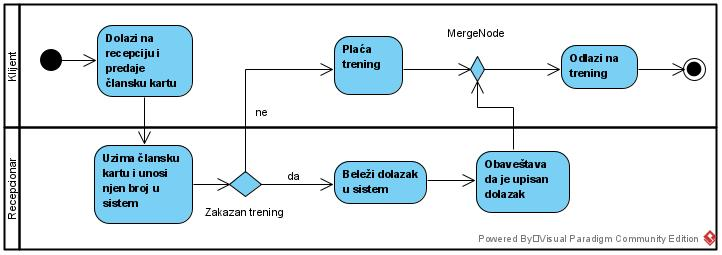
\includegraphics[scale=0.55]{sections/images/dijagram_aktivnosti_evidencije_prisustva.jpg}
\end{center}
\caption{Dijagram aktivnosti evidencije dolaska na trening}
\label{fig:kontekst}
\end{figure}

\end{document}